\chapter{Исследовательский раздел}

В данном разделе будут приведены: пример работы программы, постановка эксперимента и сравнительный анализ алгоритмов на основе полученных данных.

\section{Демонстрация работы программы}


На рисунке \ref{img:program} представлена демонстрация работы разработанного программного обеспечения, а именно показаны результаты сортировки массива $[3, 5, -3, 1, 2, 4, -6, 2]$.  
\clearpage

\includeimage
{program} % Имя файла без расширения (файл должен быть расположен в директории inc/img/)
{f} % Обтекание (без обтекания)
{h} % Положение рисунка (см. figure из пакета float)
{1\textwidth} % Ширина рисунка
{Демонстрация работы программы при сортировке массива} % Подпись рисунка

\clearpage


\section{Технические характеристики}

Технические характеристики компьютера, на котором проводился замерный эксперимент:
\begin{itemize}
	\item процессор Intel Core i5-10400F (6 ядер) \cite{intel};
	\item 16 Гб оперативная память DDR4;
	\item операционная система Windows 10 Pro \cite{windows}.
\end{itemize}

Во время проведения исследования компьютер был нагружен только системными приложениями и целевой программой.

\section{Время выполнения реализаций алгоритмов}

Результаты замеров времени выполнения реализаций алгоритмов сортировок приведены в таблицах \ref{tbl:time_measurements} -- \ref{tbl:time_measurements_rand}.
Замеры времени проводились на массивах одного размера и усреднялись для каждого набора одинаковых экспериментов.

В таблицах \ref{tbl:time_measurements} -- \ref{tbl:time_measurements_rand} используются следующие обозначения: 
\begin{itemize}
	\item Блочная --- реализация алгоритма блочной сортировки;
	\item Быстрая --- реализация алгоритма быстрой сортировки;
	\item Выбором --- реализация алгоритма сортировки выбором.
\end{itemize}

\begin{table}[h]
	\begin{center}
		\begin{threeparttable}
			\captionsetup{justification=raggedright,singlelinecheck=off}
			\caption{Время работы реализации алгоритмов на неотсортированных массивах (в мс)}
			\label{tbl:time_measurements}
			\begin{tabular}{|c|c|c|c|}
				\hline
				Размер массива & Блочная & Быстрая & Выбором \\
				\hline
				100 &$ 0.15625 $&$ 0.15625 $&$ 0.3125 $\\
				\hline
				200 &$ 0.46875 $&$ 0.15625 $&$ 0.78125 $\\
				\hline
				300 &$ 0.46875 $&$ 0.3125 $&$ 1.71875 $\\
				\hline
				400 &$ 0.78125 $&$ 0.3125 $&$ 3.4375 $\\
				\hline
				500 &$ 0.9375 $&$ 0.46875 $&$ 5.15625 $\\
				\hline
				600 &$ 1.40625 $&$ 0.625 $&$ 9.375 $\\
				\hline
				700 &$ 1.40625 $&$ 0.9375 $&$ 12.03125 $\\
				\hline
				800 &$ 1.71875 $&$ 0.9375 $&$ 14.6875 $\\
				\hline
				900 &$ 1.875 $&$ 1.25 $&$ 17.65625 $\\
				\hline
				1000 &$ 3.125 $&$ 1.26875 $&$ 21.71875 $\\
				\hline
			\end{tabular}
		\end{threeparttable}
	\end{center}
\end{table}

\begin{table}[h]
	\begin{center}
		\begin{threeparttable}
			\captionsetup{justification=raggedright,singlelinecheck=off}
			\caption{Время работы реализации алгоритмов на отсортированных в обратном порядке массивах (в мс)}
			\label{tbl:time_measurements_sorted}
			\begin{tabular}{|c|c|c|c|}
				\hline
				Размер массива & Блочная & Быстрая & Выбором \\
				\hline
				100 &$ 0.15625 $&$ 0.3125 $&$ 0.15625 $\\
				\hline
				200 &$ 0.15625 $&$ 1.25 $&$ 0.78125 $\\
				\hline
				300 &$ 0.46875 $&$ 2.8125 $&$ 2.1875 $\\
				\hline
				400 &$ 0.625 $&$ 4.53125 $&$ 3.4375 $\\
				\hline
				500 &$ 0.625 $&$ 6.5625 $&$ 5.625 $\\
				\hline
				600 &$ 0.78125 $&$ 9.53125 $&$ 7.65625 $\\
				\hline
				700 &$ 1.09375 $&$ 12.3475 $&$ 10.78125 $\\
				\hline
				800 &$ 1.09375 $&$ 16.5625 $&$ 13.59375 $\\
				\hline
				900 &$ 1.25 $&$ 19.375 $&$ 17.34375 $\\
				\hline
				1000 &$ 1.40625 $&$ 24.21875 $&$ 21.71875 $\\
				\hline
			\end{tabular}
		\end{threeparttable}
	\end{center}
\end{table}

\begin{table}[h]
	\begin{center}
		\begin{threeparttable}
			\captionsetup{justification=raggedright,singlelinecheck=off}
			\caption{Время работы реализации алгоритмов на отсортированных массивах (в мс)}
			\label{tbl:time_measurements_rand}
			\begin{tabular}{|c|c|c|c|}
				\hline
				Размер массива & Блочная & Быстрая & Выбором \\
				\hline
				100 &$ 0.15625 $&$ 0.46875 $&$ 0.15625 $\\
				\hline
				200 &$ 0.15625 $&$ 1.5625 $&$ 0.78125 $\\
				\hline
				300 &$ 0.46875 $&$ 3.90625 $&$ 2.5 $\\
				\hline
				400 &$ 0.625 $&$ 7.03125 $&$ 3.28125 $\\
				\hline
				500 &$ 0.78125 $&$ 9.21875 $&$ 5.3125 $\\
				\hline
				600 &$ 0.78125 $&$ 13.28125 $&$ 8.125 $\\
				\hline
				700 &$ 0.9375 $&$ 18.4375 $&$ 10.625 $\\
				\hline
				800 &$ 1.40625 $&$ 24.0625 $&$ 14.0625 $\\
				\hline
				900 &$ 1.25 $&$ 28.28125 $&$ 17.5 $\\
				\hline
				1000 &$ 1.40625 $&$ 34.375 $&$ 21.875 $\\
				\hline
			\end{tabular}
		\end{threeparttable}
	\end{center}
\end{table}

\clearpage
На рисунках \ref{pic:random} -- \ref{pic:sorted} изображены графики зависимостей времени выполнения реализаций сортировок от размеров массивов.

\begin{figure}[H]
	\centering
	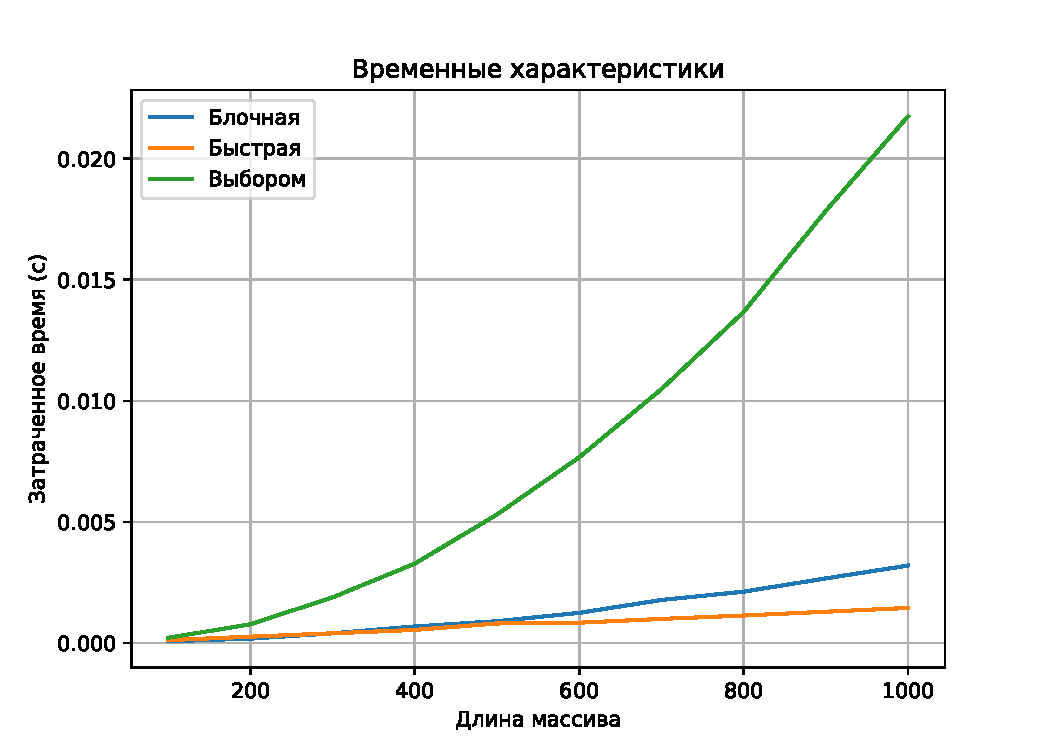
\includegraphics[scale=0.62]{assets/plots/cpu-random.pdf}
	\caption{Сравнение реализаций алгоритмов по времени выполнения на неотсортированных массивах}
	\label{pic:random}
\end{figure}

\newpage

\begin{figure}[H]
	\centering
	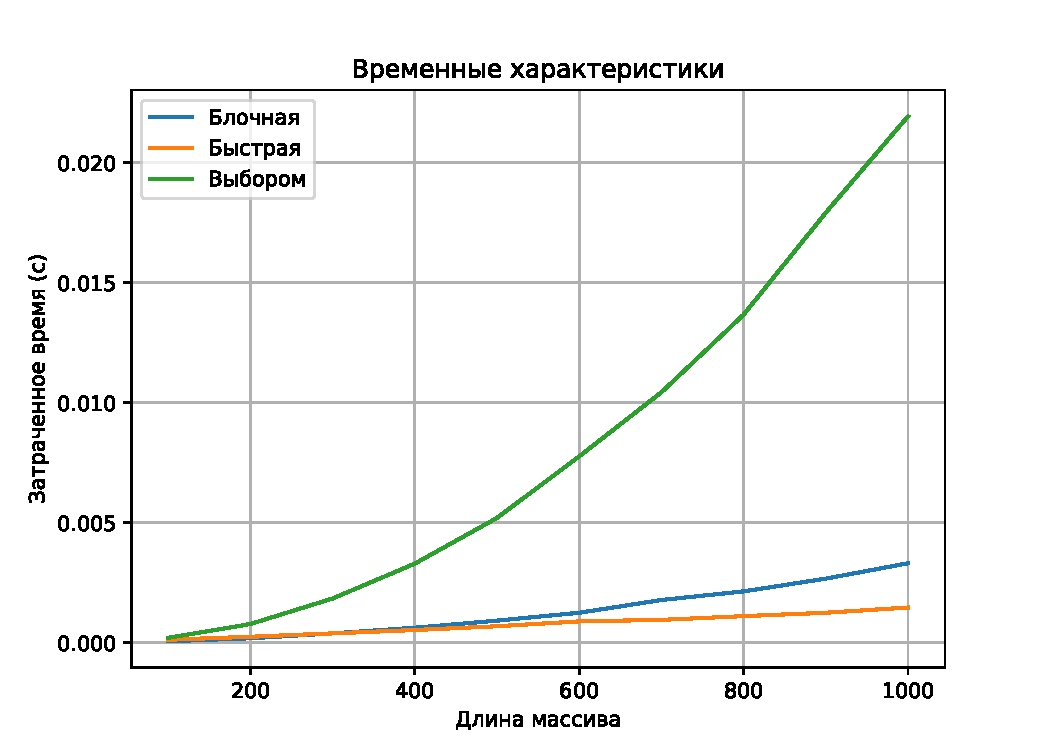
\includegraphics[scale=0.62]{assets/plots/cpu-reversed.pdf}
	\caption{Сравнение реализаций алгоритмов по времени выполнения на отсортированных в обратном порядке массивах}
	\label{pic:reversed}
\end{figure}

\newpage

\begin{figure}[H]
	\centering
	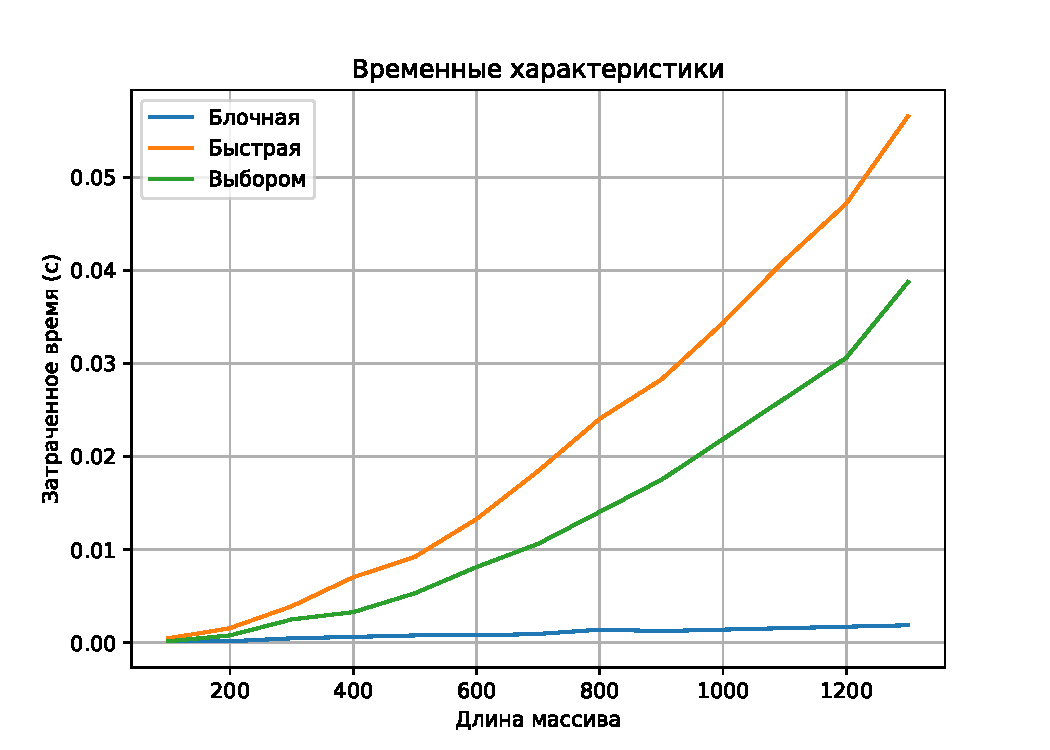
\includegraphics[scale=0.62]{assets/plots/cpu-sorted.pdf}
	\caption{Сравнение реализаций алгоритмов по времени выполнения на отсортированных массивах}
	\label{pic:sorted}
\end{figure}

\clearpage


\section{Характеристики по памяти}

Введем следующие обозначения:
\begin{itemize}
	\item $n$ --- длина массива, который необходимо отсортировать $arr$;
	\item $size()$ --- функция, вычисляющая размер в байтах;
	\item $int$ --- целочисленный тип данных;
	\item $float$ --- вещественный тип данных.
\end{itemize}

Максимальное требование по памяти реализации алгоритма Шелла складывается из 5 локальных переменных типа $int$, адреса возврата $int$, возвращаемого значения (ссылки) и рассчитывается по формуле \eqref{mem:shell}.
\begin{equation}
	\label{mem:shell}
	f_{memshell} = 6 \cdot size(int) + size(float *).
\end{equation}

Аналогично, реализация алгоритма гномьей сортировки максимально требует памяти под 2 локальные переменные типа $int$, адрес возврата $int$, возвращаемое значение (ссылку), т.~о. требования по памяти рассчитываются по формуле \eqref{mem:gnome}.
\begin{equation}
	\label{mem:gnome}
	f_{memgnome} = 3 \cdot size(int) + size(float *).
\end{equation}

Максимальное требование реализации алгоритма пирамидальной сортировки по памяти формируется из 3 локальных переменных типа $int$, адреса возврата $int$, возвращаемого по ссылке значения, при этом максимальная глубина рекурсии подпрограммы \textit{heapify} равна $\log_2 N$. 
В подпрограмме \textit{heapify} используются 3 локальных переменных типа $int$, а для вызова в нее необходимо передать массив по ссылке и 2 переменные типа $int$. 
Память требуемая реализацией алгоритма пирамидальной сортировки рассчитывается по формуле \eqref{mem:heap}.
\begin{equation}
	\label{mem:heap}
	f_{heap} = 3 \cdot size(int) + size(float *) + \log_2 N (6 \cdot size(int) + size(float *)).
\end{equation}

\section*{Вывод}

В результате замеров времени выполнения реализаций различных алгоритмов было выявлено, что для массивов длины 9000, отсортированных в обратном порядке, реализация алгоритма Шелла по времени оказалась в 2.6 раза лучше, чем реализация гномьей сортировки, и в 4.5 раза лучше реализации пирамидальной сортировки. 
В свою очередь, реализация гномьей сортировки оказалась лучше в 1.7 раз по времени выполнения, чем реализация пирамидальной сортировки.
Что соответствует теоретической оценке трудоемкости. 
Поскольку алгоритм Шелла по теоретической оценке трудоемкости в худшем случае выигрывает по константе гномью сортировку, $O(\frac{32}{3}N^2)$ и $O(\frac{23}{2}N^2)$ соответственно, при этом алгоритм пирамидальной сортировки, обладая теоретической оценкой трудоемкости $O(\frac{87}{2} N \log_2N)$, из-за большой константы проигрывает остальным, хоть и обладает меньшей скоростью роста.

Для отсортированных массивов длинной 9000 реализация гномьей сортировки оказалась лучше по времени в 9 раза, чем реализация алгоритма Шелла, и в 42 раза лучше, чем реализация пирамидальной сортировки. 
В свою очередь, реализация пирамидальной сортировки на отсортированных массивах, оказалась хуже в 4.5 раза, чем реализации алгоритма Шелла по времени выполнения. 
Что соответствует теоретической оценке трудоемкости.
Поскольку в лучшем случае алгоритм гномьей сортировки обладает наименьшей асимптотической оценкой и малой константой $O(7N)$. А алгоритм Шелла выигрывает алгоритм пирамидальной сортировки по константе, $O(10 N \log_2N)$ и $O(29 N \log_2N)$ соответственно.

Для случайно упорядоченных массивов длинной 9000 реализация гномьей сортировки оказалась лучше по времени в 1.4 раза, чем реализация алгоритма Шелла, и в 5.3 раза лучше, чем реализация пирамидальной сортировки. 
В свою очередь, реализация пирамидальной сортировки на случайно упорядоченных массивах, оказалась хуже в 3.9 раз, чем реализации алгоритма Шелла по времени выполнения.

При этом меньше всего памяти требует реализация гномьей сортировки, а больше всего --- реализация пирамидальной сортировки.

Стоит заметить, что для обратно упорядоченных массивов длинной менее 2500, реализация гномьей сортировки показывала лучшие результаты. 
На случайно упорядоченных массивах, гномья сортировка хоть и оказалась эффективней, но обладая большей скоростью роста, при больших длинах массивов она окажется менее эффективной, чем сортировка Шелла и пирамидальная. 
То же касается и пирамидальной сортировки, за счет большой константы, она показала худший результат во всех случаях, но поскольку асимптотическая оценка этого алгоритма меньше остальных для случайно упорядоченных и обратно упорядоченных массивов, данная реализация покажет лучшую эффективность по времени при гораздо больших длинах массивов.